\documentclass[conference]{IEEEtran}
\IEEEoverridecommandlockouts
% The preceding line is only needed to identify funding in the first footnote. If that is unneeded, please comment it out.
\usepackage{cite}
\usepackage{amsmath,amssymb,amsfonts}
\usepackage{algorithmic}
\usepackage{graphicx}
\usepackage{textcomp}
\usepackage{xcolor}
\usepackage{graphicx}
\usepackage{cite}
\usepackage{url}
\usepackage{amsmath}
\usepackage{amssymb}
\usepackage{epstopdf}
\usepackage{multirow}
\usepackage{hhline}
\graphicspath{ {figure/} }
\usepackage[numbers]{natbib}
\def\BibTeX{{\rm B\kern-.05em{\sc i\kern-.025em b}\kern-.08em
    T\kern-.1667em\lower.7ex\hbox{E}\kern-.125emX}}

\begin{document}

\title{Neural Network Implementation on FPGA}

\author{\IEEEauthorblockN{Hongxin Kong}
\IEEEauthorblockA{\textit{Department of Electrical and Computer Engineering} \\
\textit{Texas A\&M University}\\
College Station, USA \\
konghongxin911@tamu.edu}
\and
\IEEEauthorblockN{Lang Feng}
\IEEEauthorblockA{\textit{Department of Electrical and Computer Engineering} \\
\textit{Texas A\&M University}\\
College Station, USA \\
flwave@tamu.edu}
}

\maketitle

\begin{abstract}
Nowadays, various of machine learning approaches emerged due to the sufficient hardware and software performance. Neural network is the most prevalent topic in machine learning. Benefitted from modern computer architectures, its powerful structure equipped it high capability in the field of regression and classification. However, due to the low difficulty of implementation, software-based neural networks are still used more frequent than hardware-based. In this paper, we try to propose a hardware-based neural network architecture for training and inference. The proposed architecture is highly configurable and implemented on field programmable gate array (FPGA).
\end{abstract}

\begin{IEEEkeywords}
neural network, hardware, FPGA
\end{IEEEkeywords}

\section{Introduction}

Recent years, with high performance hardware and software emerging, machine learning approaches become more practical to implement. A typical area of machine learning, neural network, becomes a popular approach for doing various of machine learning tasks. With the demand of high performance and low overhead neural networks, sometimes software-based neural networks cannot satisfy the requirements, thus, many researches focus on implementing neural networks by hardware~\cite{hwsurvey}. 

Neural networks are networks with neurons and connections. One each of the connection, there is weight. The input data will propagate from the input to all the neurons with the weights and activation functions. By doing this, a nonlinear mapping from the input data to the output data is realized, thus, it can be used as classification or regression. There are mainly two parts in neural networks. One is reference, which means forward propagation of the input. When a neural network is well built, users can do reference to get their results. Another is training. During training, the weights of the neural networks will converge to the values that make the neural networks perform the similar pattern as the given learning reference outputs. This is also called learning. Benefit from this property, when users give the neural networks enough inputs and corresponding correct outputs, neural networks can automatically learn the pattern by updating weights using backpropagation.

Field-programmable gate array (FPGA) is a prevalent platform for hardware implementation. Its agility property gives ditital hardware designers chances to emulate their designs before tapeout. Moreover, due to the convenience for updating, some designs even use FPGA as a target platform for implementations. In our work, we will use FPGA as a platform for verify our ideas. Theoretically, our design can also be manufactured as application-specific integrated circuit (ASIC).

Neural networks on hardware have been explored long time ago, but it is still not widly used. Neural networks which are based on FPGA are also proposed by many researchers~\cite{FPGAbook}. Some works like~\cite{hytnh17,seok02} proposed FPGA-based neural network implementations and have advantages over normal software-based implementations. However, there are still many spaces for improving current FPGA-based neural network architectures. We plan to improve the neural network architecture based on the work~\cite{hytnh17}.

In the conclusion, our work has the following contributions:
\begin{itemize}
\item Proposed a real system that can fully finish the training tasks of the fully connected neural networks. 
\item A detailed implementation of hardware neural networks with configurable layers and neurons.
\end{itemize}

In the following sections, we first discuss some previous works in Section~\ref{sec:prev}, then introduce the fully connected neural networks used in our work in Section~\ref{sec:nn}. The system platform is proposed in Section~\ref{sec:sys}, and the FPGA-based neural network architecture is proposed in Section~\ref{sec:fpgann}. We will then discuss the detailed implementation details in Section~\ref{sec:impl}. Finally, Section~\ref{sec:exp} and Section~\ref{sec:ccl} show the experiment results and conclusions.

\section{Previous works}
\label{sec:prev}
Neural networks were proposed long time ago~\cite{nn88,nn89,nn91}, but they are not widely used because of the limited computing resources. Neural networks need great amount of memory and high performance parallel computing resources which are not usually valid in the last century. 

In this century, with the increased computer performance and GPU computing, neural networks almost master the area of artificial intelligence and machine learning. More and more neural networks structures are proposed, like convolutional neural networks~\cite{convnet} and generative adversarial networks~\cite{gan}.  It is shown that general central processing unit is no longer suitable for neural network operations, but highly paralleled computing, like GPU, can benefit more to neural networks.

Furthermore, researchers have explored to use specific hardware for neural networks, like tensor processing unit~\cite{tpu,tpu2} and spike neural networks~\cite{spike}.  The hardware based neural networks show great performance comparing to regular software based neural networks. 

Field programmable gate array (FPGA) is a modern platform for hardware design. Its high configurability enable engineers or researchers quickly implement their hardware designs. Works related with FPGA-based neural networks have been proposed~\cite{hytnh17,seok02}. However, due to the FPGA resource limitation, previous works usually implement a fixed trained neural networks with only inference function. This will degrade the value of FPGA and make the design impractical. Therefore, in our work, unlike~\cite{hytnh17}, we implement a configurable fully connected neural network that can be applied with configurable hyperparameters. Meanwhile, our neural network can also be trained in FPGA. 

\section{Fully Connected Neural Network}
\label{sec:nn}
In this section, we briefly introduce the reference and training of the fully connected neural network. A fully connected neural network is composed with neurons of many layers. Assume the input layer is layer 0, then the output of each neurons in layer i (i$>$0) will connect to the inputs of all the neurons in layer i+1. 

For reference, for neuron i, it will first multiply each input with the corresponding weight, add all the results, and input the added result into an activation function. In this paper, we use sigmoid function as our activation function. The overall equation for reference is: 
\begin{equation}
y=\phi(\Sigma_{j}(x_i w_{ij}))
\end{equation}
Where j is the index of the neuron in the previous layer, and $w_{ij}$ is the weight from neuron j to neuron i. $\phi$ is the sigmoid function: $\phi(v)=\frac{1}{1+exp(-v)}$.

For training, it will be more complex. The training of fully connected neural network follows the backpropogation of the gradient decent. for each neuron j, the weight change will always follow:
\begin{equation}
\Delta w_{ji}=\eta \delta _j x_i
\end{equation}
Where j is the neuron index of the next layer, $\eta$ is the gradient decent ratio, and $\delta _j$ is:
\begin{equation}
\delta _j= y_j(1-y_j) \times error
\label{equ:delta}
\end{equation}
The $\phi \prime$ is the difference of the active function, and the error is:
\begin{equation}
error=\Sigma_{k}(\delta _k w_k j)
\end{equation}
Where k is the index of neuron j's next layer's neuron. If neuron j is at the output layer, the error is:
\begin{equation}
error=-(d_j-y_j)
\end{equation}
Where $d_j$ is the correct output of neuron j.

By using the equations above, we can update the weight and realize the training.

\section{System platform}
\label{sec:sys}

Our proposed neural network architecture is implemented in an SoC platform shown in Figure~\ref{fig:sys}. Due to the limited memory size of FPGA, additional processor with Linux system is used for transferring data. To train a neural network, the system will follow these steps:
\begin{itemize}
\item Linux system allocates a part of memory in the kernel.
\item Processor loads the training set and testing set from files to allocated memory.
\item FPGA reads the training set's data by the physical address through AXI bus.
\item FPGA trains the neural network.
\item FPGA reads the testing set's data, does inference, and returns the result to the memory.
\end{itemize}

\begin{figure}[!hbt]
	\centering
	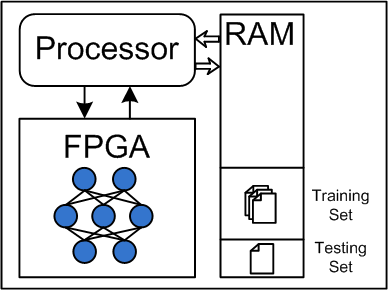
\includegraphics[width=0.3\textwidth]{sys.png}
	\caption{System platform.}
	\label{fig:sys}
\end{figure}

\section{FPGA-based Neural Network Architecture}
\label{sec:fpgann}

Given a neural network structure, theoretically it can always be implemented by hardware logical circuits. However, each FPGA only has limited hardware resources. Some previous works, like~\cite{hytnh17}, only implement a specific neural network structure for one kind of use. For our work, we propose a neural network structure with configurable hyperparameters that can be trained given the dataset. 

For each hardware-based neuron, it should have two parts: reference and training. Therefore, we design the neuron as shown in Figure~\ref{fig:neuron}.

\begin{figure}[!hbt]
	\centering
	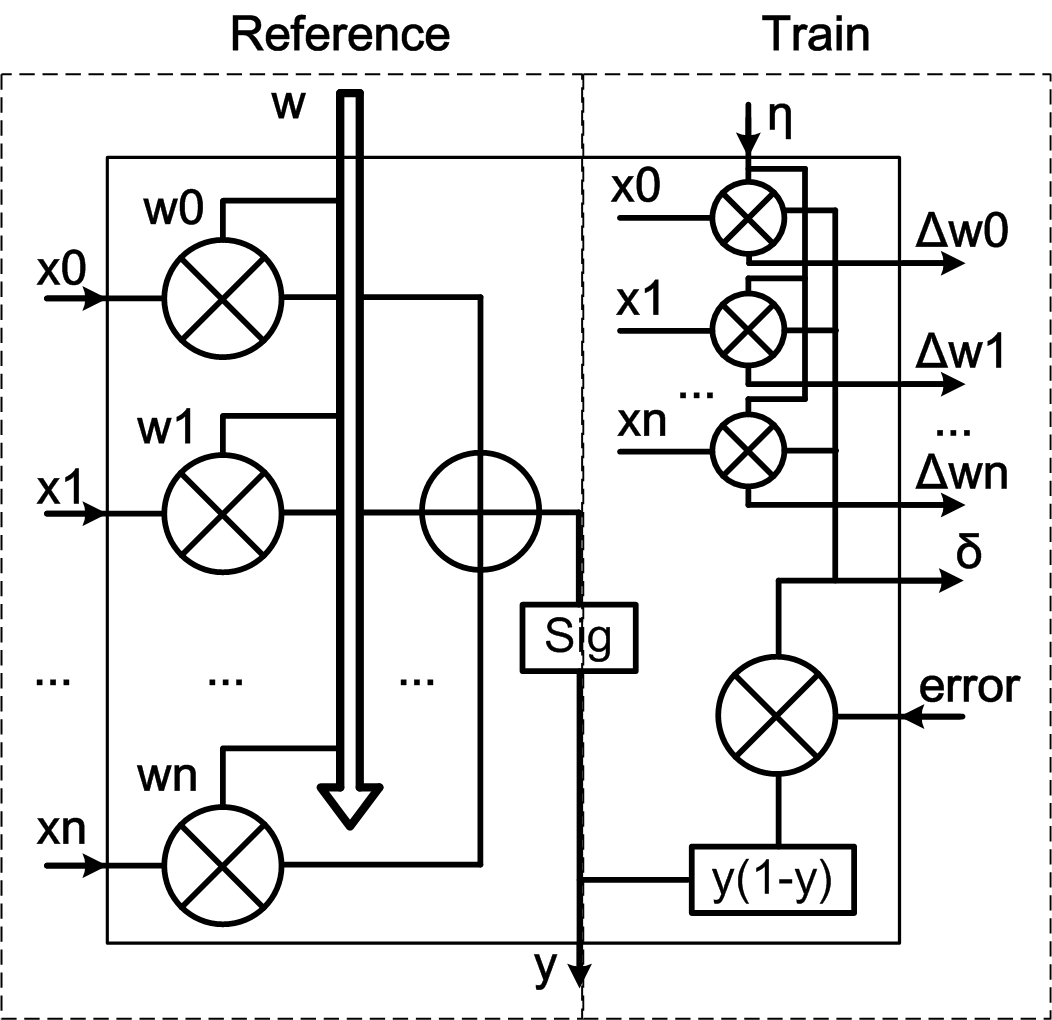
\includegraphics[width=0.4\textwidth]{neuron.png}
	\caption{The architecture of one neuron in the FPGA.}
	\label{fig:neuron}
\end{figure}

In Figure~\ref{fig:neuron}, circles with $\times$ means multiply, circles with $+$ means add, x is the input of the neuron, w is the weight, $\eta$ is the gradent decent ratio, $\Delta w$ is the difference of the weight, and $\delta$ is the $\delta$ in Equation~\ref{equ:delta}.  

Besides the architecture for the neuron, we also need an global architecture for network. We illustrate it in Figure~\ref{fig:global}.

\begin{figure}[!hbt]
	\centering
	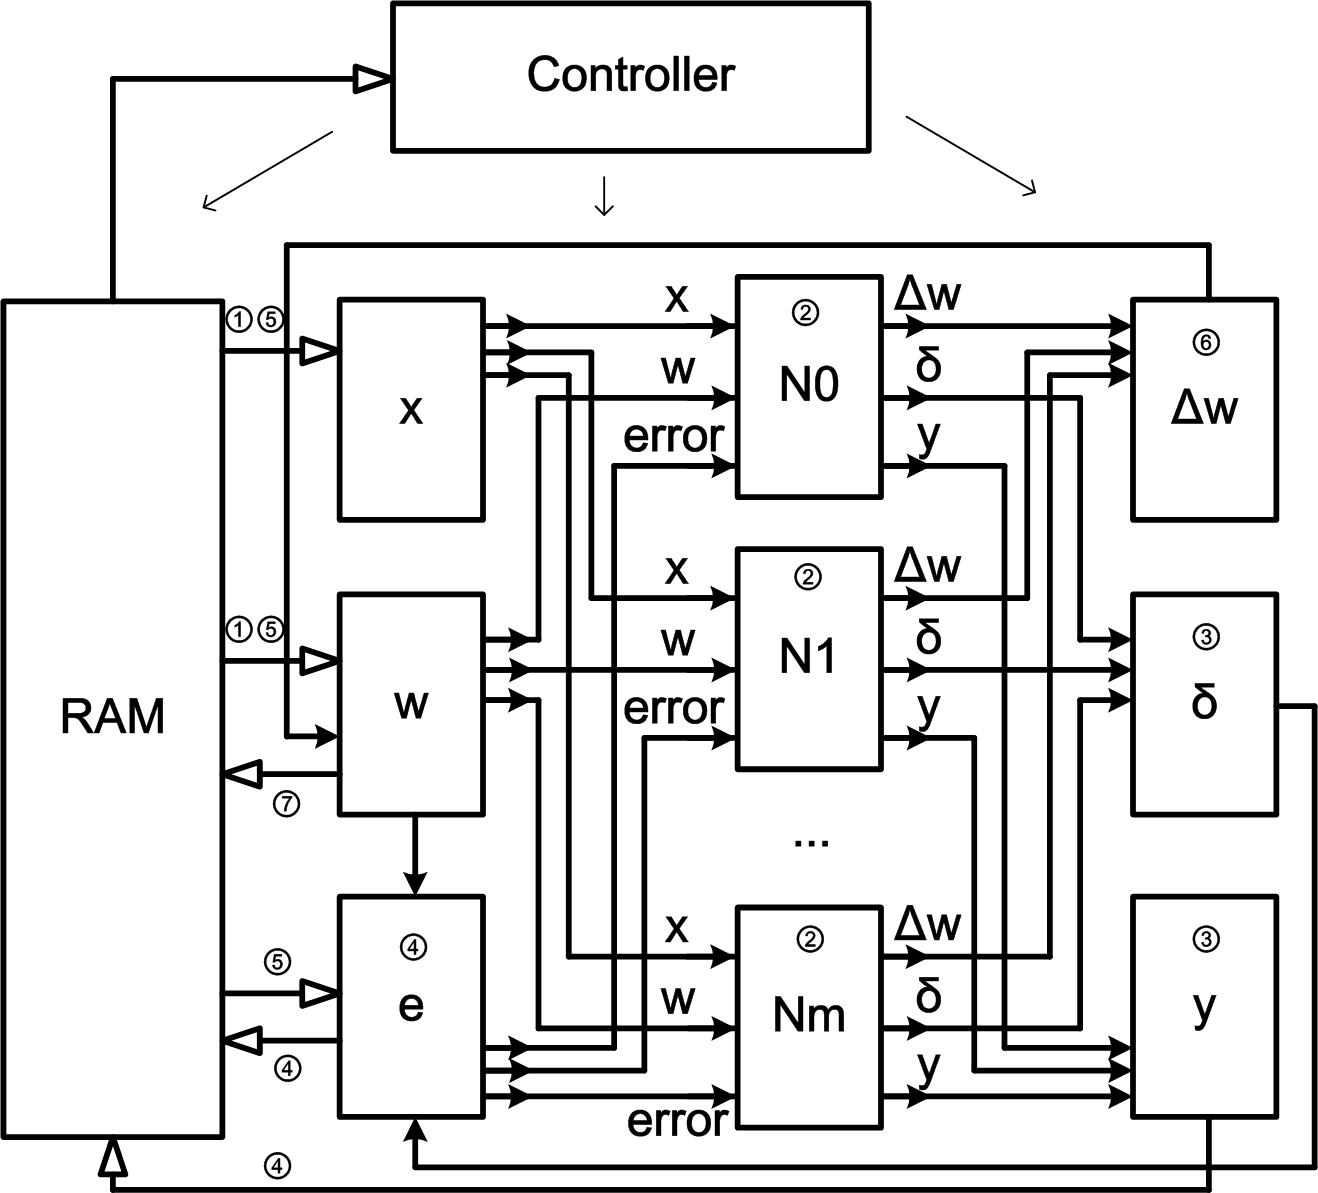
\includegraphics[width=0.47\textwidth]{global.png}
	\caption{The global architecture of the FPGA design.}
	\label{fig:global}
\end{figure}

The rectangles with "Nx" in Figure~\ref{fig:global} represent the neurons illustrated in Figure~\ref{fig:neuron}. Moreover, except controller and RAM, other rectangles represent the buffer for specific data. The RAM is the memory of the processor, which can be accessed by AXI bus from FPGA side.

The number of the neuron instances, m, can be configured by user before synthesis, according to the hardware resources of the FPGA. However, the number of neuron instances will not affect the training and reference of the target neural network structure required by the user. We will get into detailed steps of the architecture.

The controller is in charge of all the processes in the FPGA.  When the training data is ready, the controller will fetch the information from RAM. The fetched information contains the target neural network structure (number of neurons, layers, etc). According to the target neural network, the data will be read from the RAM and trained.

When we do the reference for one layer, FPGA will perform as the following steps:
\begin{itemize}
\item 1. FPGA will read the input data and weight from RAM into the buffer.
\item 2. FPGA will choose at most m neurons which haven't done reference in this layer, and input the data and weights to each neuron instance that stands for a neuron in the layer. Each neuron instance will then output the results.
\item 3. The results will be stored in the buffers.
\item 4. The output of each neuron, y, will be used to calculate the error of the neuron along with weights. The error and output will be stored in the RAM.
\item Do the above steps until all the neurons in this layer are referenced. Then move to next layer.
\end{itemize}

If we need to train the neural network, we need first do the reference. After that, the errors are stored in the RAM. FPGA will do the following for at most m neurons in one layer:
\begin{itemize}
\item 5. FPGA will load the recorded data, weights and errors to the buffers.
\item 6. FPGA will calculate the differences of weights. 
\item 7. The results will be used to update the weights, and the weights will be stored back to RAM.
\item Do the above steps until all the neurons in this layer are trained. Then move to previous layer.
\end{itemize}

Note that although we use limited number of neuron instances (in the case above, we use m instances), the instances can change their roles to many neurons in the user defined neural networks. This means, the proposed architecture can realize the training of fully connected neural networks with any kinds of hyperparameters.

\section{Implementation}
\label{sec:impl}

We use Intel DE1-SoC board for implementation. In this board, it contains an ARM processor and an FPGA. 

\subsection{Data Transferring}
FPGA has limited memory, thus, we use the memory (DRAM) of the ARM processor, which is 1GB. In the Linux system running on the ARM processor, we allocate 512MB memory for data transferring between DRAM and FPGA. 

To realize this, we have to use kernel memory but not user memory, since we cannot get the physical address of the user memory directly. The first step to do this is to write a kernel module. We need the source code of the Linux system for DE1-SoC, which can be found in~\cite{linux}. In the kernel module, we need to use "kmalloc" to allocate 512MB memory and display the physical address of it, which can be realized in kernel module. The start address of our case is 0x0e800000. 

After the memory is allocated, we use the first 128MB for training and testing data, the next 256MB for weights, and the last 128MB for other information. Before we start training, the training and testing data will be loaded beforehand, by a user level program. This user level program will map the memory starting from 0x0e800000 to a pointer, then read the dataset and write the data into the first 128MB.

On FPGA side, FPGA will access the memory through the physical address. It will need AXI bus to access. Since we use Intel FPGA, we can create a system platform by using Platform Designer in Quartus 17.1. Benefit from the build-in modules, we can first build the complete ARM to FPGA basic system and then manually split the bus between JTAG and AXI in the source code, and thus, we can use the same way that JTAG uses to control the AXI bus interface. The waveform of read from and write to AXI bus is shown in Figure~\ref{fig:axir} and Figure~\ref{fig:axiw}. As we can see, it needs about 10 FPGA clock cycles to access the memory. 

\begin{figure}[!hbt]
	\centering
	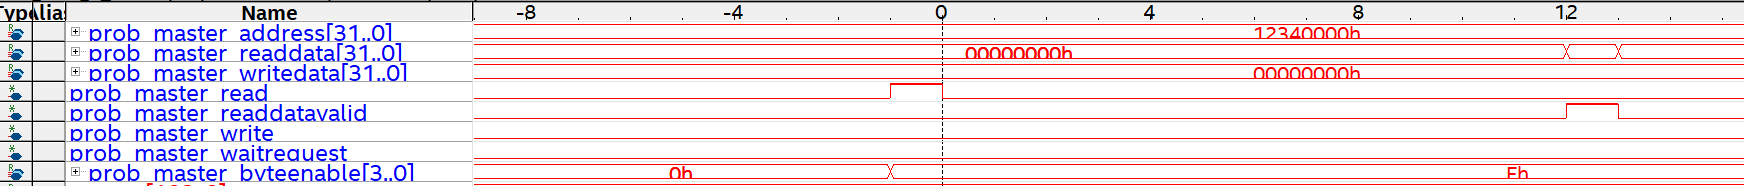
\includegraphics[width=0.47\textwidth]{axiread.png}
	\caption{The waveform of reading 4 bytes through AXI bus.}
	\label{fig:axir}
\end{figure}

\begin{figure}[!hbt]
	\centering
	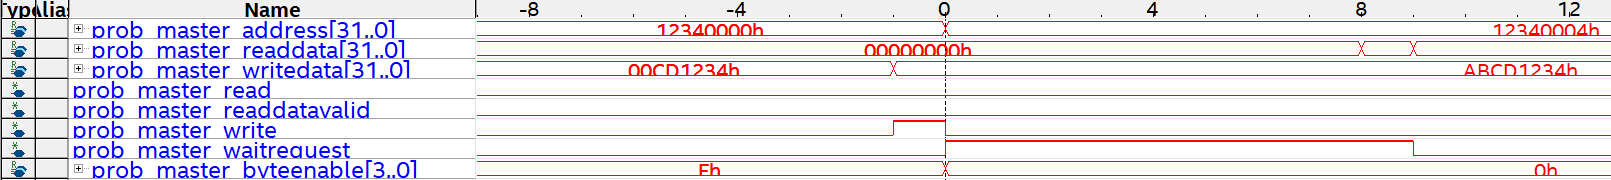
\includegraphics[width=0.47\textwidth]{axiwrite.png}
	\caption{The waveform of writing 4 bytes through AXI bus.}
	\label{fig:axiw}
\end{figure}

\subsection{FPGA-based Neural Network Implementation}

\subsubsection{Neuron}

Since hardware circuits has no flexibility, which means their structure cannot be changed while using them, so we can only design fixed number of neurons and use them for the whole neural networks. In our design, for each neuron, we allocate 32 inputs with each of them 32-bit. This is enough for most cases. For the activation function, we use ReLu, which is very easy for hardware circuit because there is not multiplication or division. The netlist of each neuron is shown in Figure~\ref{fig:nnnl}.

\begin{figure}[!hbt]
	\centering
	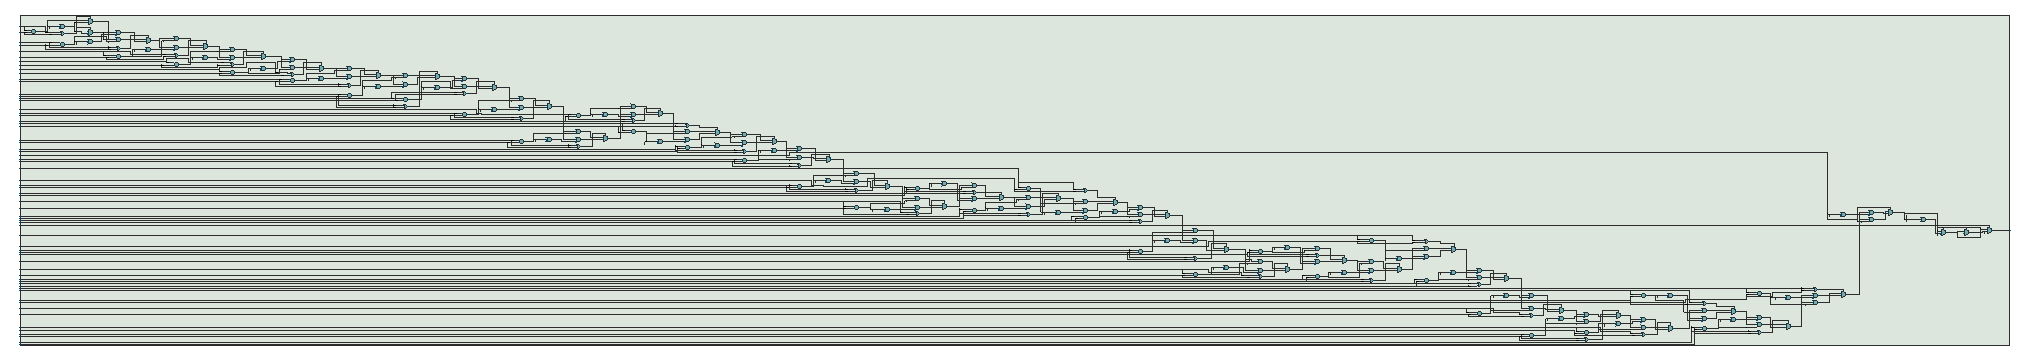
\includegraphics[width=0.47\textwidth]{neuron_nl.png}
	\caption{The netlist of one neuron.}
	\label{fig:nnnl}
\end{figure}

As we can see, the synthesized netlist has long critical path. The reason is the result of the neuron is calculated by the sum of each weighted input, where the sum is a serial process. Therefore, we cannot allocate numerous input ports due to the reason that this will incur a longer critical path and thus, incur timing error.

\subsubsection{Data Format}

In our implementation, each input of a neuron is 32-bit. We use 1's complement number, which means, the most significant bit indicates if the number is positive (0) or negative (1). The reminding bits are for the value of the number. The output of the neuron is:
\begin{equation}
y=\phi(\Sigma_{j}(x_i w_{ij}))
=\phi(x_0 w_{00}+x_1 w_{01}+...)
\end{equation}
To do the application, the multiplier of our design will get 2 1's complement inputs, and output 2's complement number to do addition. After the addition, we use ReLu as the activation function, so it will transform all the positive 2's complement to 1's complement as the next layer's input, and transform all the negative number to 0.

\subsubsection{Controller}

Note that due to some technical reasons, we haven't implemented the design of the training part. We only implemented the inference part. 

The controller is implemented by a finite state machine (FSM). As shown in Figure~\ref{fig:fsm}, The FSM has 6 state, which are IDLE, LOADIN, LOADW, LOADB, TRANS, FINISH. We will introduce each state in detail.

\begin{figure}[!hbt]
	\centering
	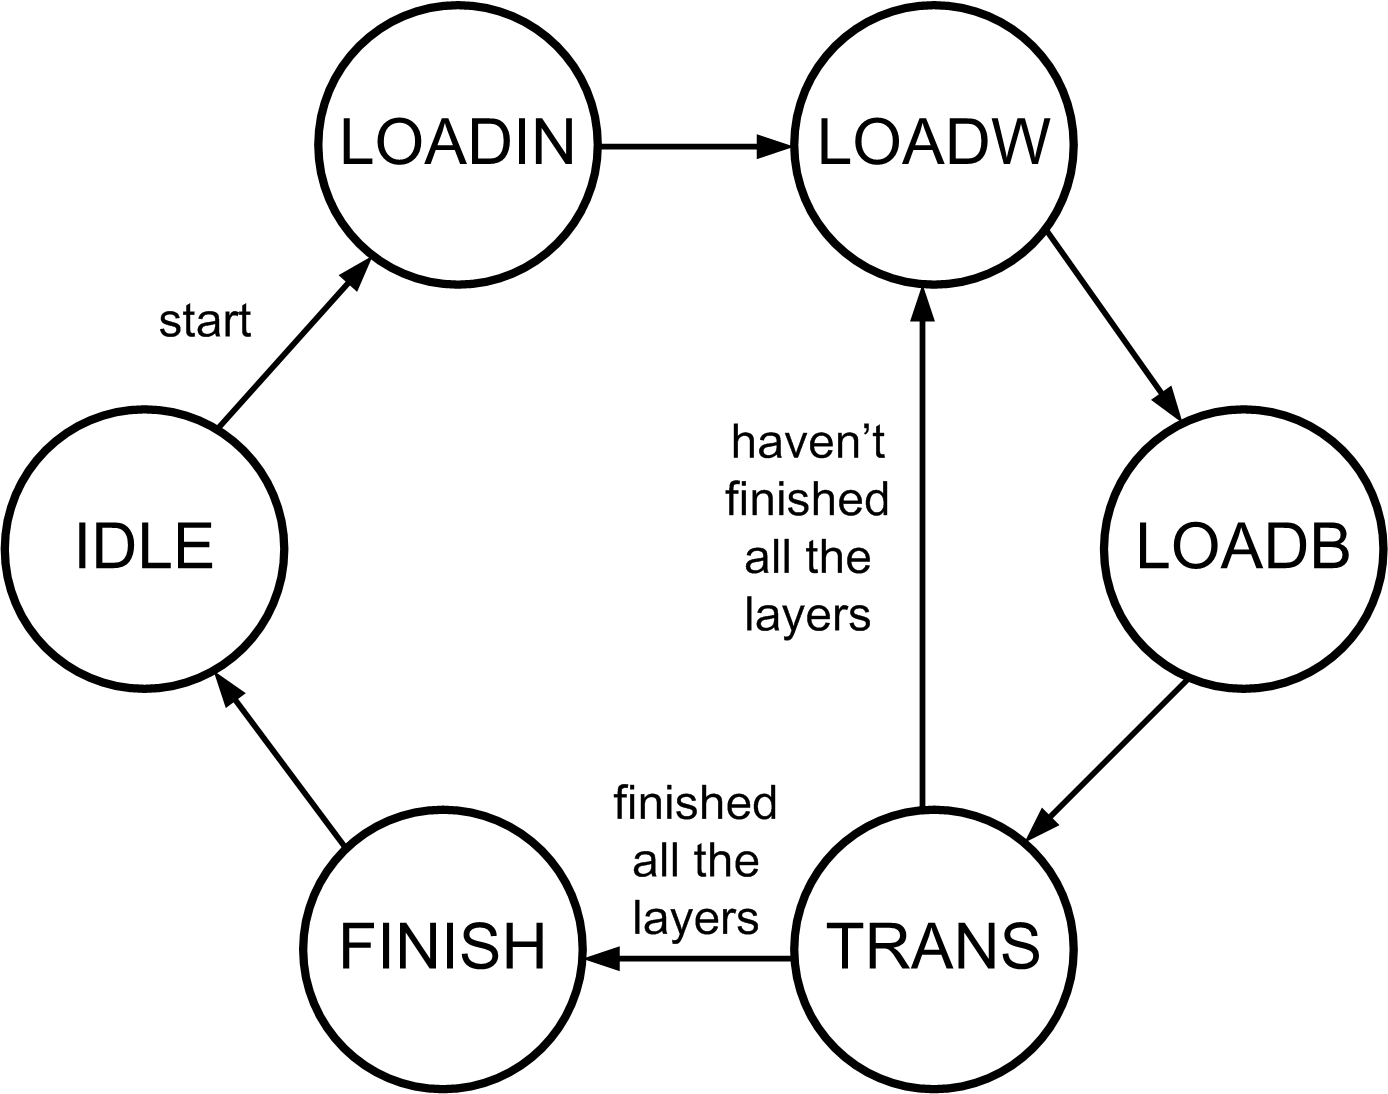
\includegraphics[width=0.42\textwidth]{fsm.png}
	\caption{The finite state machine in the controller.}
	\label{fig:fsm}
\end{figure}

The FSM will start as IDLE. In this state, the controller will wait for the start signal. Once it receives, FSM will go to LOADIN state.

In LOADIN state, the controller will load the input data into the buffer, and that is the input of the neuron instances. After this, controller will get into LOADW state and then LOADB state, which are to load the first layer's weights and biases. Note that we designed the interface between the controller and the AXI to load the data.

After all the data is loaded, controller will get into TRANS state. This state is to let data transfer inside all the neurons, get the output, and transfer the output to the input buffer. Note that the input buffer originally contains the input data, but after there is output of the first layer, the data in the input buffer is replaced by the output, which represent the input of the second layer. After this, state will change to LOADW and LOADB again, to read the second layer's weights and biases.

After all the layers are calculated, controller will get into FINISH state and output the final data. Since we transfer the output of the neuron to the input side, and load weights and biases layer by layer, we only need one layer of the neurons, and this can make our design flexible and user can train as many layers as they configured, only if the number of neurons in each layer is in the range of the neuron instances in FPGA.

\section{Experiments and Results}
\label{sec:exp}
\subsection{Experiment Setup}

We use Intel DE1-SoC board to evaluate our design. The board contains an ARM Cortex-A9 processor, 1GB DRAM, and a Cyclone V FPGA. The software for implementing the hardware is Quartus, and the software for simulation is Modelsim. The dataset for training and inference is MNIST dataset. One example of the data in the dataset is shown in Figure~\ref{fig:data}. This is the example of number "0", where white space is encoded in 0, and line is encoded in 1. The size of the figure is 32*32. When implementation, we decrease the resolution of each row by 2, which means, it changes to 32*16. This is better for hardware since the hardware has limit bandwidth. Also, this won't decrease the accuracy much. The neural network we used has 3 layers, where the number of the neurons are 32, 30 and 10. 

\begin{figure}[!hbt]
	\centering
	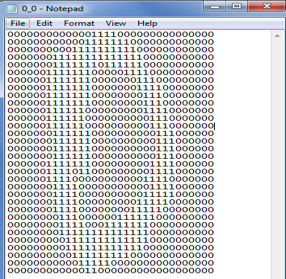
\includegraphics[width=0.25\textwidth]{data.png}
	\caption{One example of the data in the dataset.}
	\label{fig:data}
\end{figure}

\subsection{Netlist}

In this part, we will propose the result of the netlist synthesized by Quartus. In Figure~\ref{fig:topnl}, it shows the netlist of the top level entity used for simulation. The database is the simulated interface that can output the data and weights. The controller is the controller we discussed in the former section. The database can be replaced by the real interface which communicated with AXI, which shown in Figure~\ref{fig:topnl2p}, which is a part of the netlist in Figure~\ref{fig:topnl2}. 

\begin{figure}[!hbt]
	\centering
	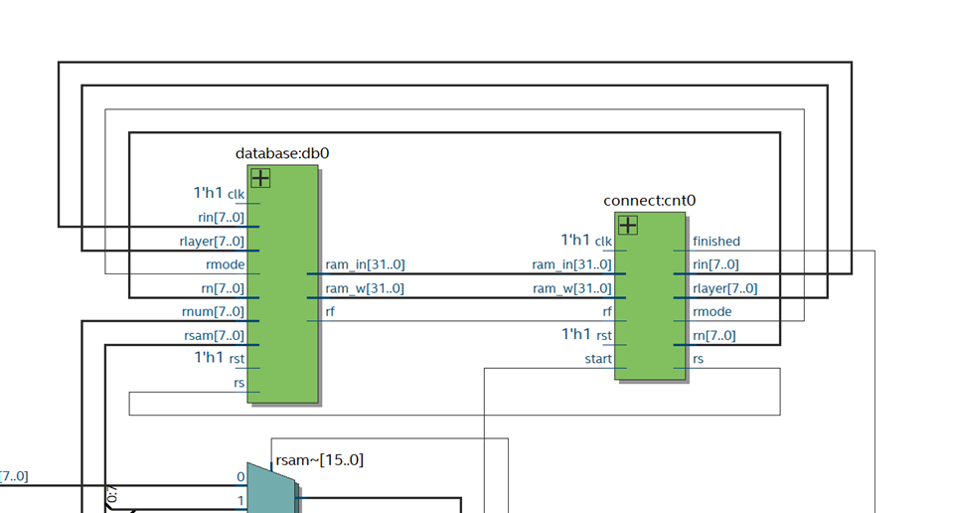
\includegraphics[width=0.4\textwidth]{topnl.png}
	\caption{The top level netlist for simulation.}
	\label{fig:topnl}
\end{figure}

In Figure~\ref{fig:topnl2p}, "read\_wbin" is the real interface interact with AXI bus and read the inputs, weights and biases. When we want to implement our design in this SoC system, we can replace the database in Figure~\ref{fig:topnl} with the part in Figure~\ref{fig:topnl2p}.

\begin{figure}[!hbt]
	\centering
	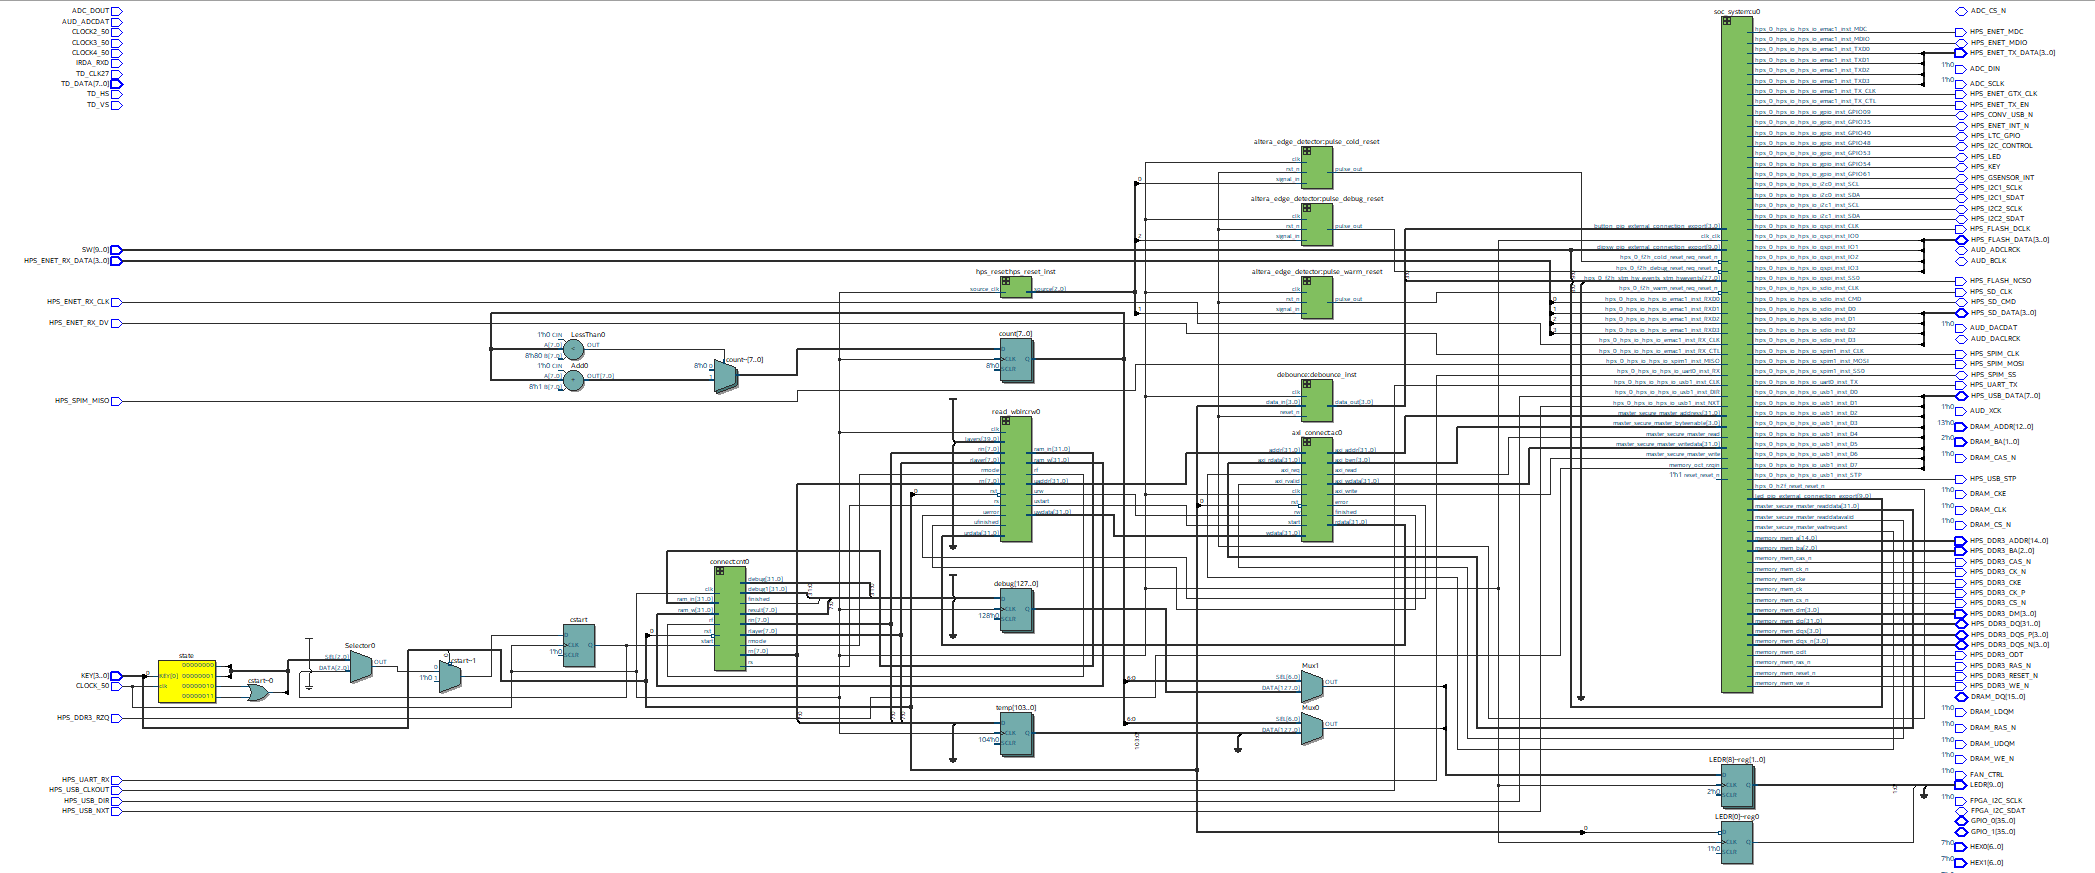
\includegraphics[width=0.4\textwidth]{topnl2.png}
	\caption{The top level netlist when using real SoC system.}
	\label{fig:topnl2}
\end{figure}

\begin{figure}[!hbt]
	\centering
	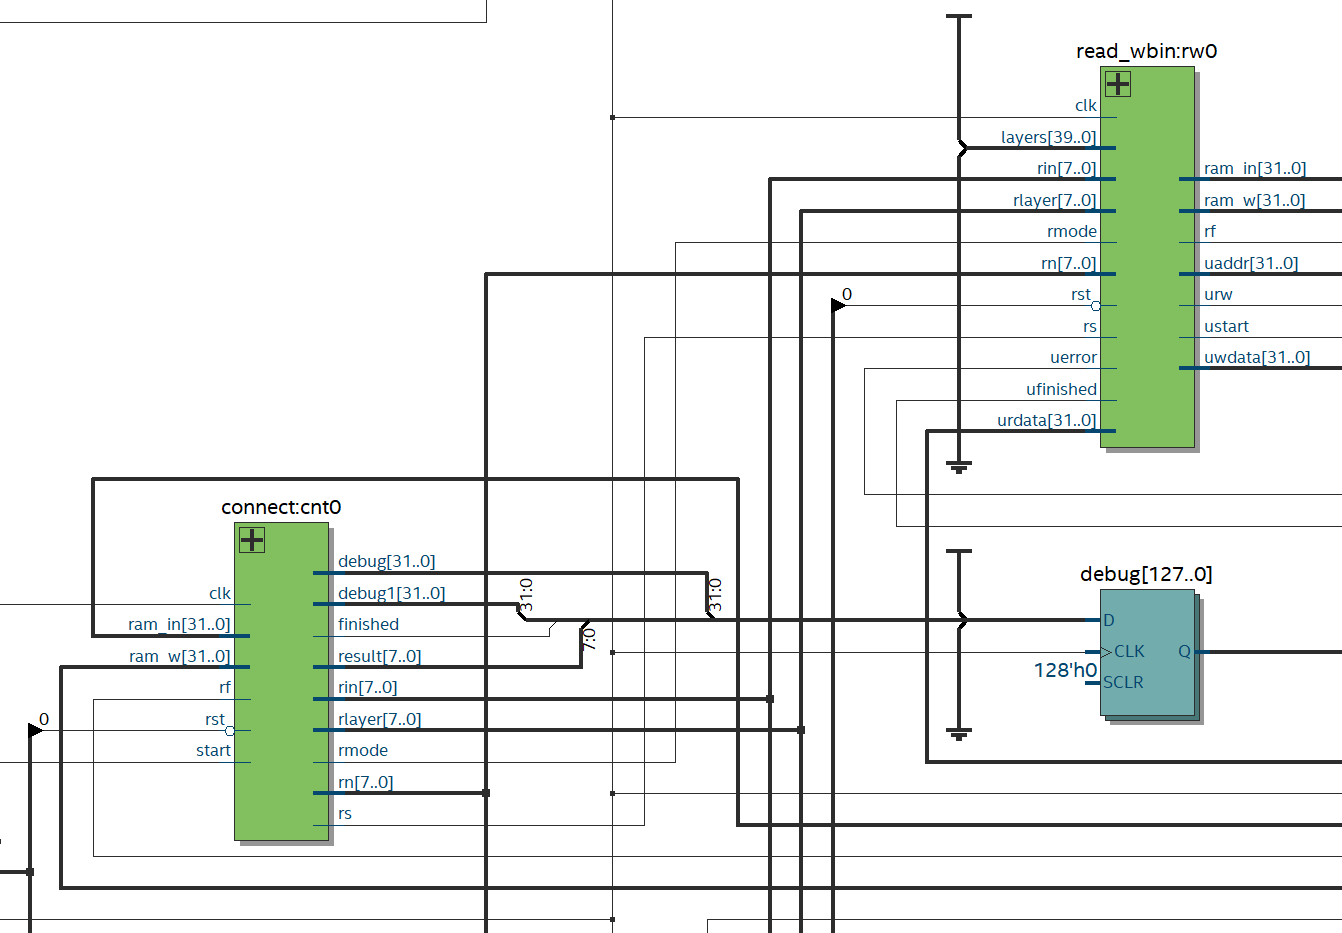
\includegraphics[width=0.4\textwidth]{topnl2p.png}
	\caption{A part of the top level netlist when using real SoC system.}
	\label{fig:topnl2p}
\end{figure}

\begin{figure*}[!hbt]
	\centering
	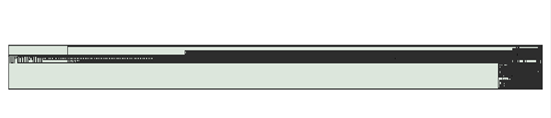
\includegraphics[width=0.6\textwidth]{ctrlnl.png}
	\caption{The netlist of the proposed controller.}
	\label{fig:ctrlnl}
\end{figure*}

Another netlist results are the netlist of the controller. We first implemented our neural network structure as it is. This means, we instantiate the same number of the neurons as the hidden layer and output layer, and connect them in the fixed way. The netlist is shown in Figure~\ref{fig:ctrlnld}. 

Then the proposed design is implemented (inference part). It is shown in Figure~\ref{fig:ctrlnl}. Note that the this figure is rotated left by 90 degree, so the critical path is still not long. As we can see, because we need register to store the output of each layer, the structure is more complicated than the directly mapped structure.

\begin{figure}[!hbt]
	\centering
	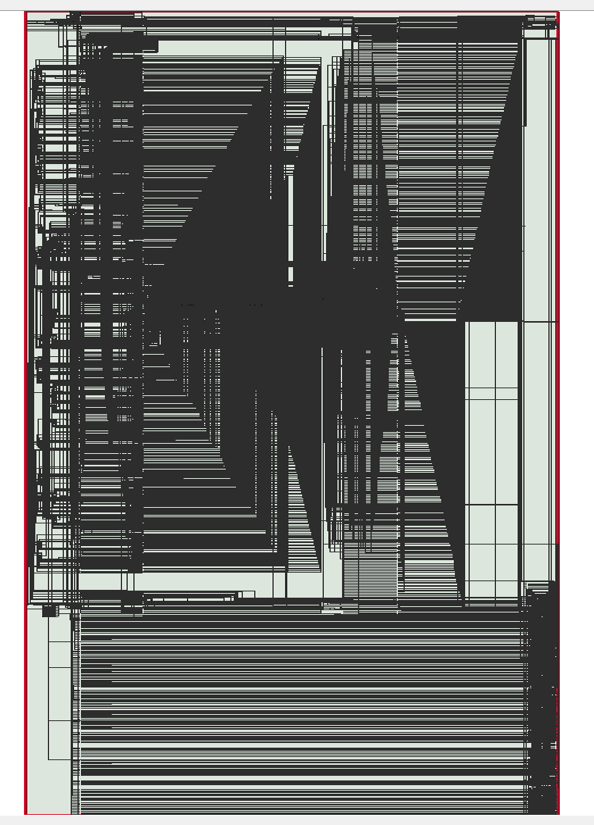
\includegraphics[width=0.2\textwidth]{ctrlnld.png}
	\caption{The netlist of the directly mapped controller.}
	\label{fig:ctrlnld}
\end{figure}

\subsection{Accuracy}

The most important challenge for hardware base neural network is the precision. Using hardware circuit cannot use as much bits as the user want. So usually we will lose precision. Fortunately, neural network is a kind of approximate computing, thus, sometimes losing precision is acceptable. However, we should also test how much accuracy it will lose.
After trained on PC, our neural network model can achieve 64\% accuracy for the 100 testing data. To compare with this, we test the same 100 data on the FPGA circuit. The result in Figure~\ref{fig:acc} shows that 59 of them are correct, which means the accuracy is 59\%. The decreasing of the accuracy is due to the precision, but it is totally acceptable.

\begin{figure}[!hbt]
	\centering
	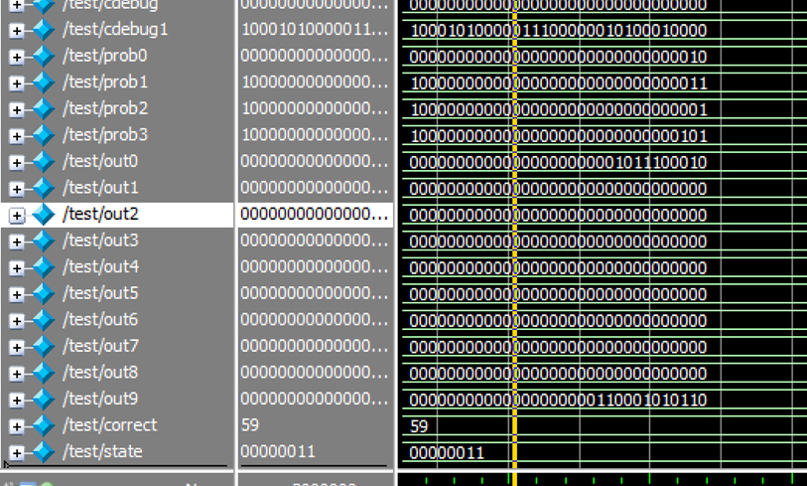
\includegraphics[width=0.4\textwidth]{accuracy.png}
	\caption{The accuracy of our design.}
	\label{fig:acc}
\end{figure}

\subsection{Latency}

Latency is the time interval between the beginning of the inference to the end. Latency is an important metrics since it affects the performance of the neural network. Nowadays, one of the bottlenecks of neural network is the time cost. Usually, neural network requires a highly parallelized system to be deployed, which can decrease the latency. FPGA is a good platform for parallel computing.
For our design, we tested the latency. Figure~\ref{fig:waveform} shows the waveform of 100 data inference. It spends about 1350000ns, so it is about 6750 FPGA clock cycles for each sample, which is also an acceptable number.

\begin{figure}[!hbt]
	\centering
	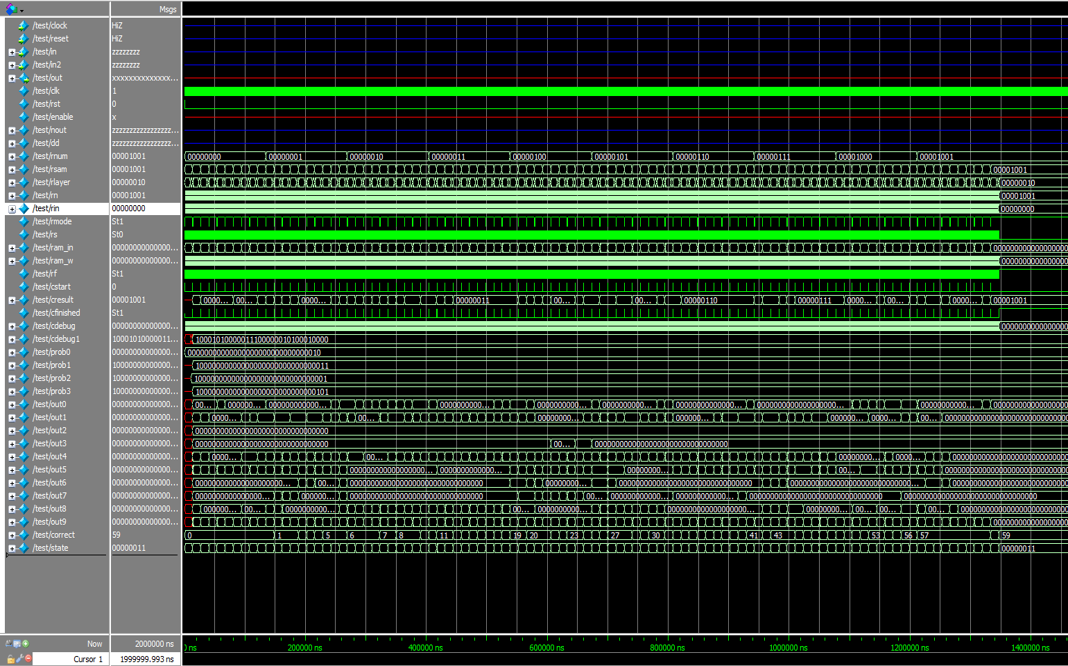
\includegraphics[width=0.4\textwidth]{latency.png}
	\caption{The waveform of 100 data inference.}
	\label{fig:waveform}
\end{figure}

\section{Conclusion}
\label{sec:ccl}

In our work, we deigned a configurable FPGA based neural network training architecture, and implemented the inference part on FPGA. The design can be used by a dynamically, which means the neural network structure and weights and biases do not need to be fixed. The accuracy does not decrease much and the latency is short. In the future, we plan to implement the training part of our design as well as more kinds of neural networks.

\section*{Appendices}
About the division of work, Hongxin Kong trained the neural network, designed the structure of each neuron, designed the data format. Lang Feng designed the controller, designed the data transfer approach, and wrote the paper.

Attached in the top zip file, there are all source codes and samples.

There are 3 zip files.

In linux\_programs.zip:
database.py can generate the data for the testbench of the simulation Verilog program.
NNtf.py can do training and write the weights and biases on PC. Use "python NNtf.py s" to train and store the weights and biases. Use "python NNtf.py l" to load the trained weights and biases and test again.
trans614.c is the ARM program to transfer weights from ARM to RAM. (This program needs a file called weights)
mymodule.ko is the system module to open 64MB RAM space for FPGA.
writeweight.py is to write the weights and biases to the file "weights".

quartus\_project\_simulation.zip is the Verilog project of the neural network simulation.
quartus\_project\_SoC.zip is the Verilog project of the data transferring interface with ARM.

\bibliographystyle{ieeetr}
 {\scriptsize \bibliography{reference}}

\end{document}
